\documentclass[12pt,a4paper]{article}
\usepackage[a4paper,left=2cm,right=2cm,top=3cm,bottom=3cm]{geometry}
\usepackage[utf8]{inputenc}
\usepackage[T1]{fontenc}
\usepackage{amsmath}
\usepackage{amssymb}
\usepackage{graphicx}
\usepackage{float}
\usepackage{nicefrac}
\usepackage[ngerman]{babel}
\title{Untersuchung Rauschverhalten\\[3ex] \small{ X-106 mit Empfindlichkeit 0...30$\mu\varepsilon$; 2. Kampagne}}

\author{Mirco Huber}




\begin{document}
	\maketitle
	\newpage

\section{Vergleich DuT 100Hz (vergossen) vs DuT 40Hz (unvergossen)}
\noindent
In einer ersten Messung wurden die DuTs erneut ''Rücken an Rücken'' belastet, sodass beide Sensoren etwa die selbe Dehnung erfahren. Die Resultate in Abb. \ref{fig:daten001} zeigen, dass die Sensoren vergleichbare Signale liefern, das Nullpunktverhalten des DuTs mit Eckfrequenz 100Hz aber stabiler erscheint.
\begin{figure}[H]
	\centering
	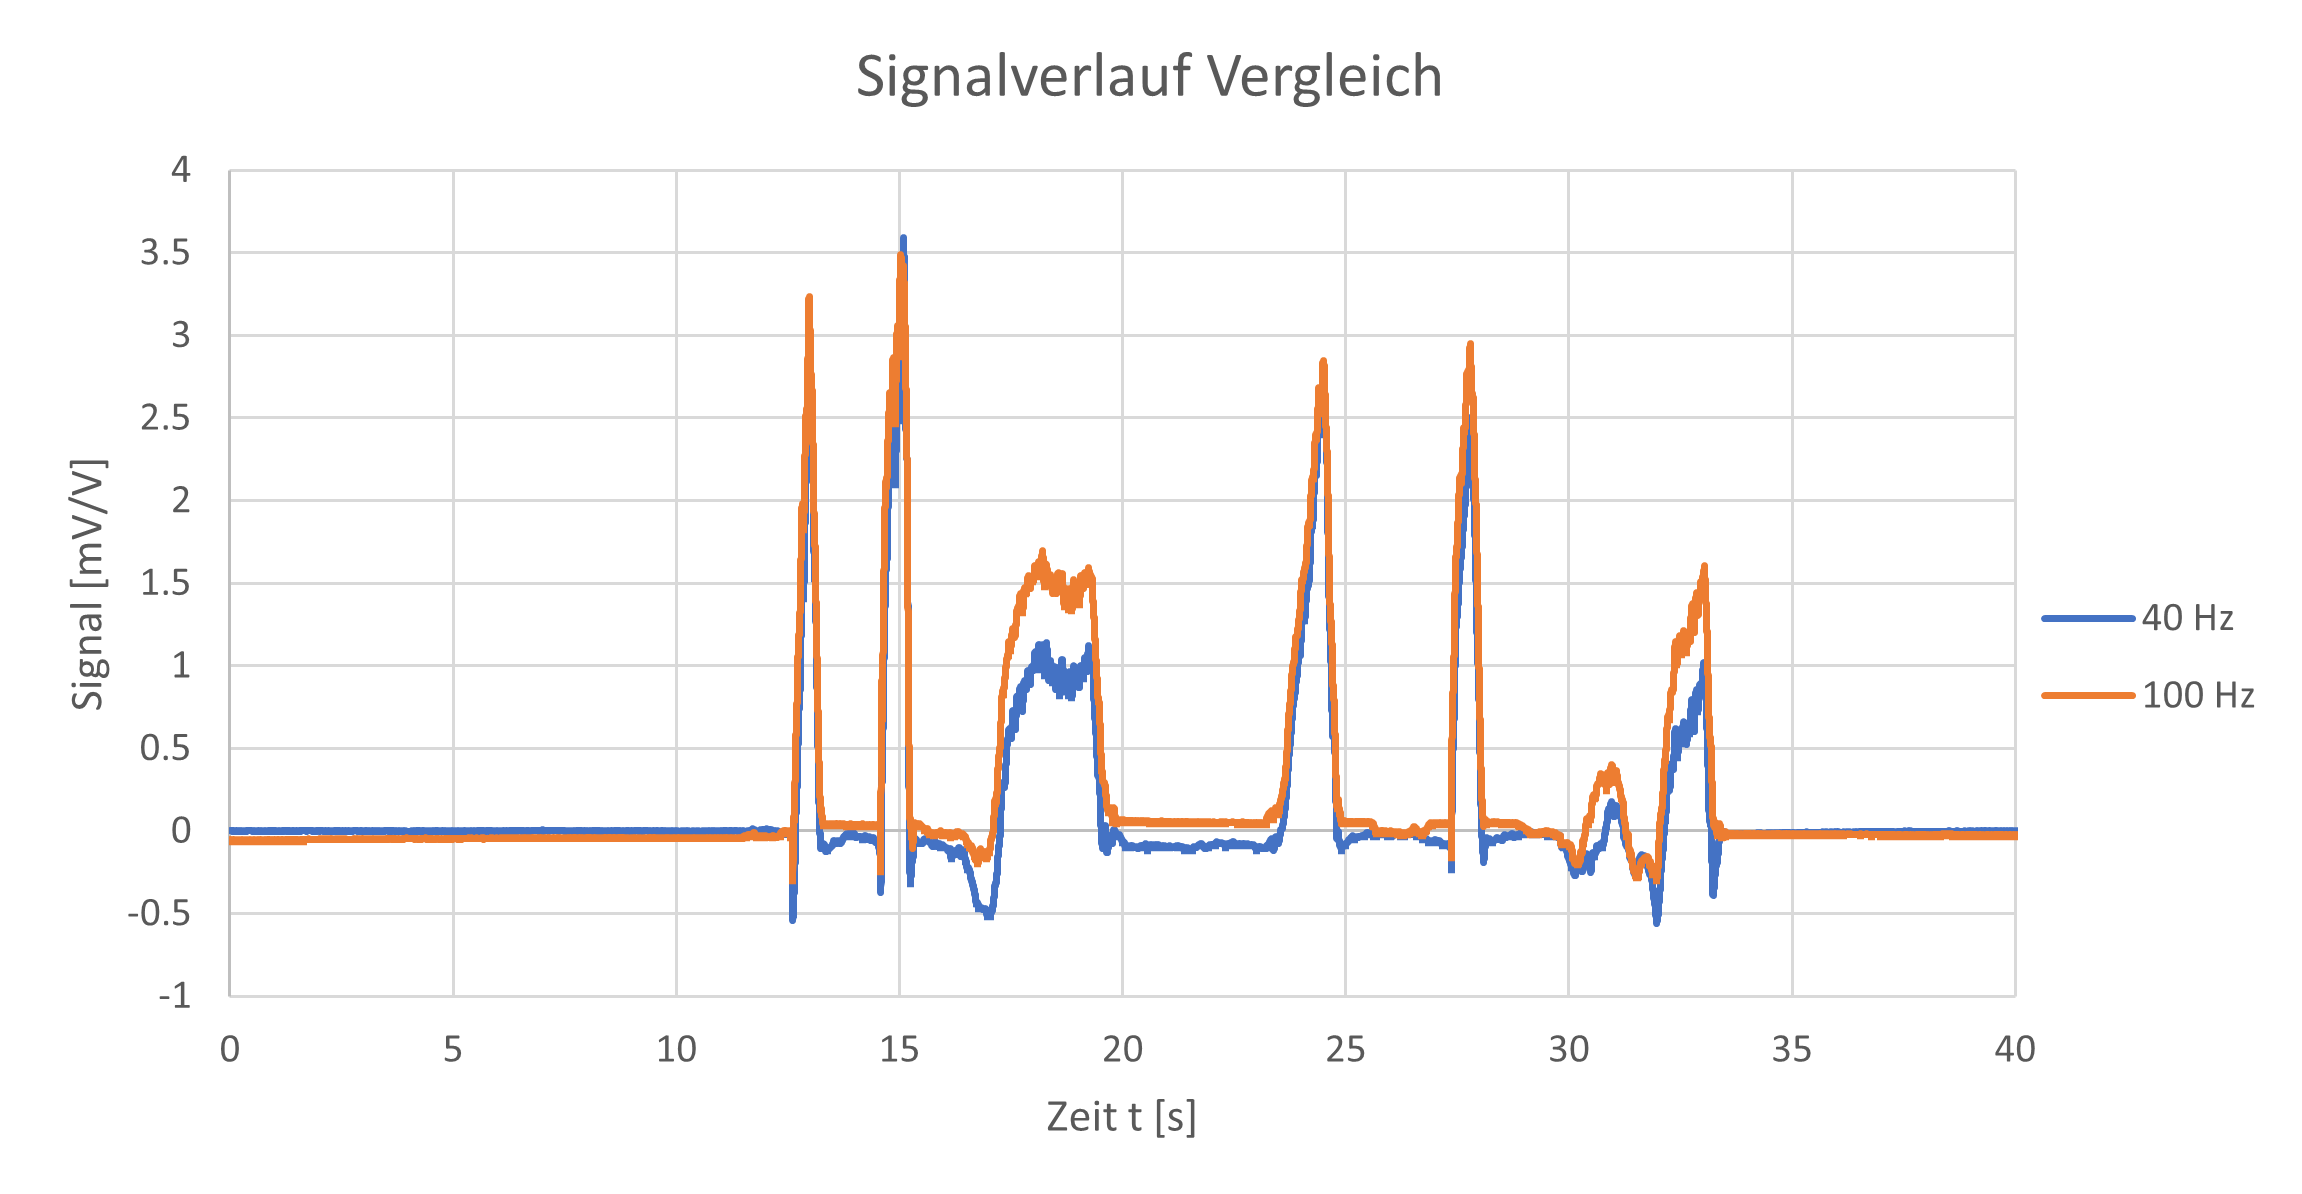
\includegraphics[width=1\linewidth]{imgs/daten_001}
	\caption{40 Hz (unvergossen) vs 100 Hz (vergossen) bei vergleichbarer Belastung}
	\label{fig:daten001}
\end{figure}
\noindent
In der Abbildung \ref{fig:daten001_NP} wird die unbelastete Phase (0...10 s) aus obiger Abbildung genauer betrachtet. Es ist zu erkennen, dass in diesem Ausschnitt das DuT mit Eckfrequenz 40Hz stabiler ist; das andere DuT zeigt einen Nullpunkt-Drift von $\sim 20\mu\varepsilon$, was bei einem FS von $2\nicefrac{mV}{V}$ rund $ 1\%$ entspricht. 
\begin{figure}[H]
	\centering
	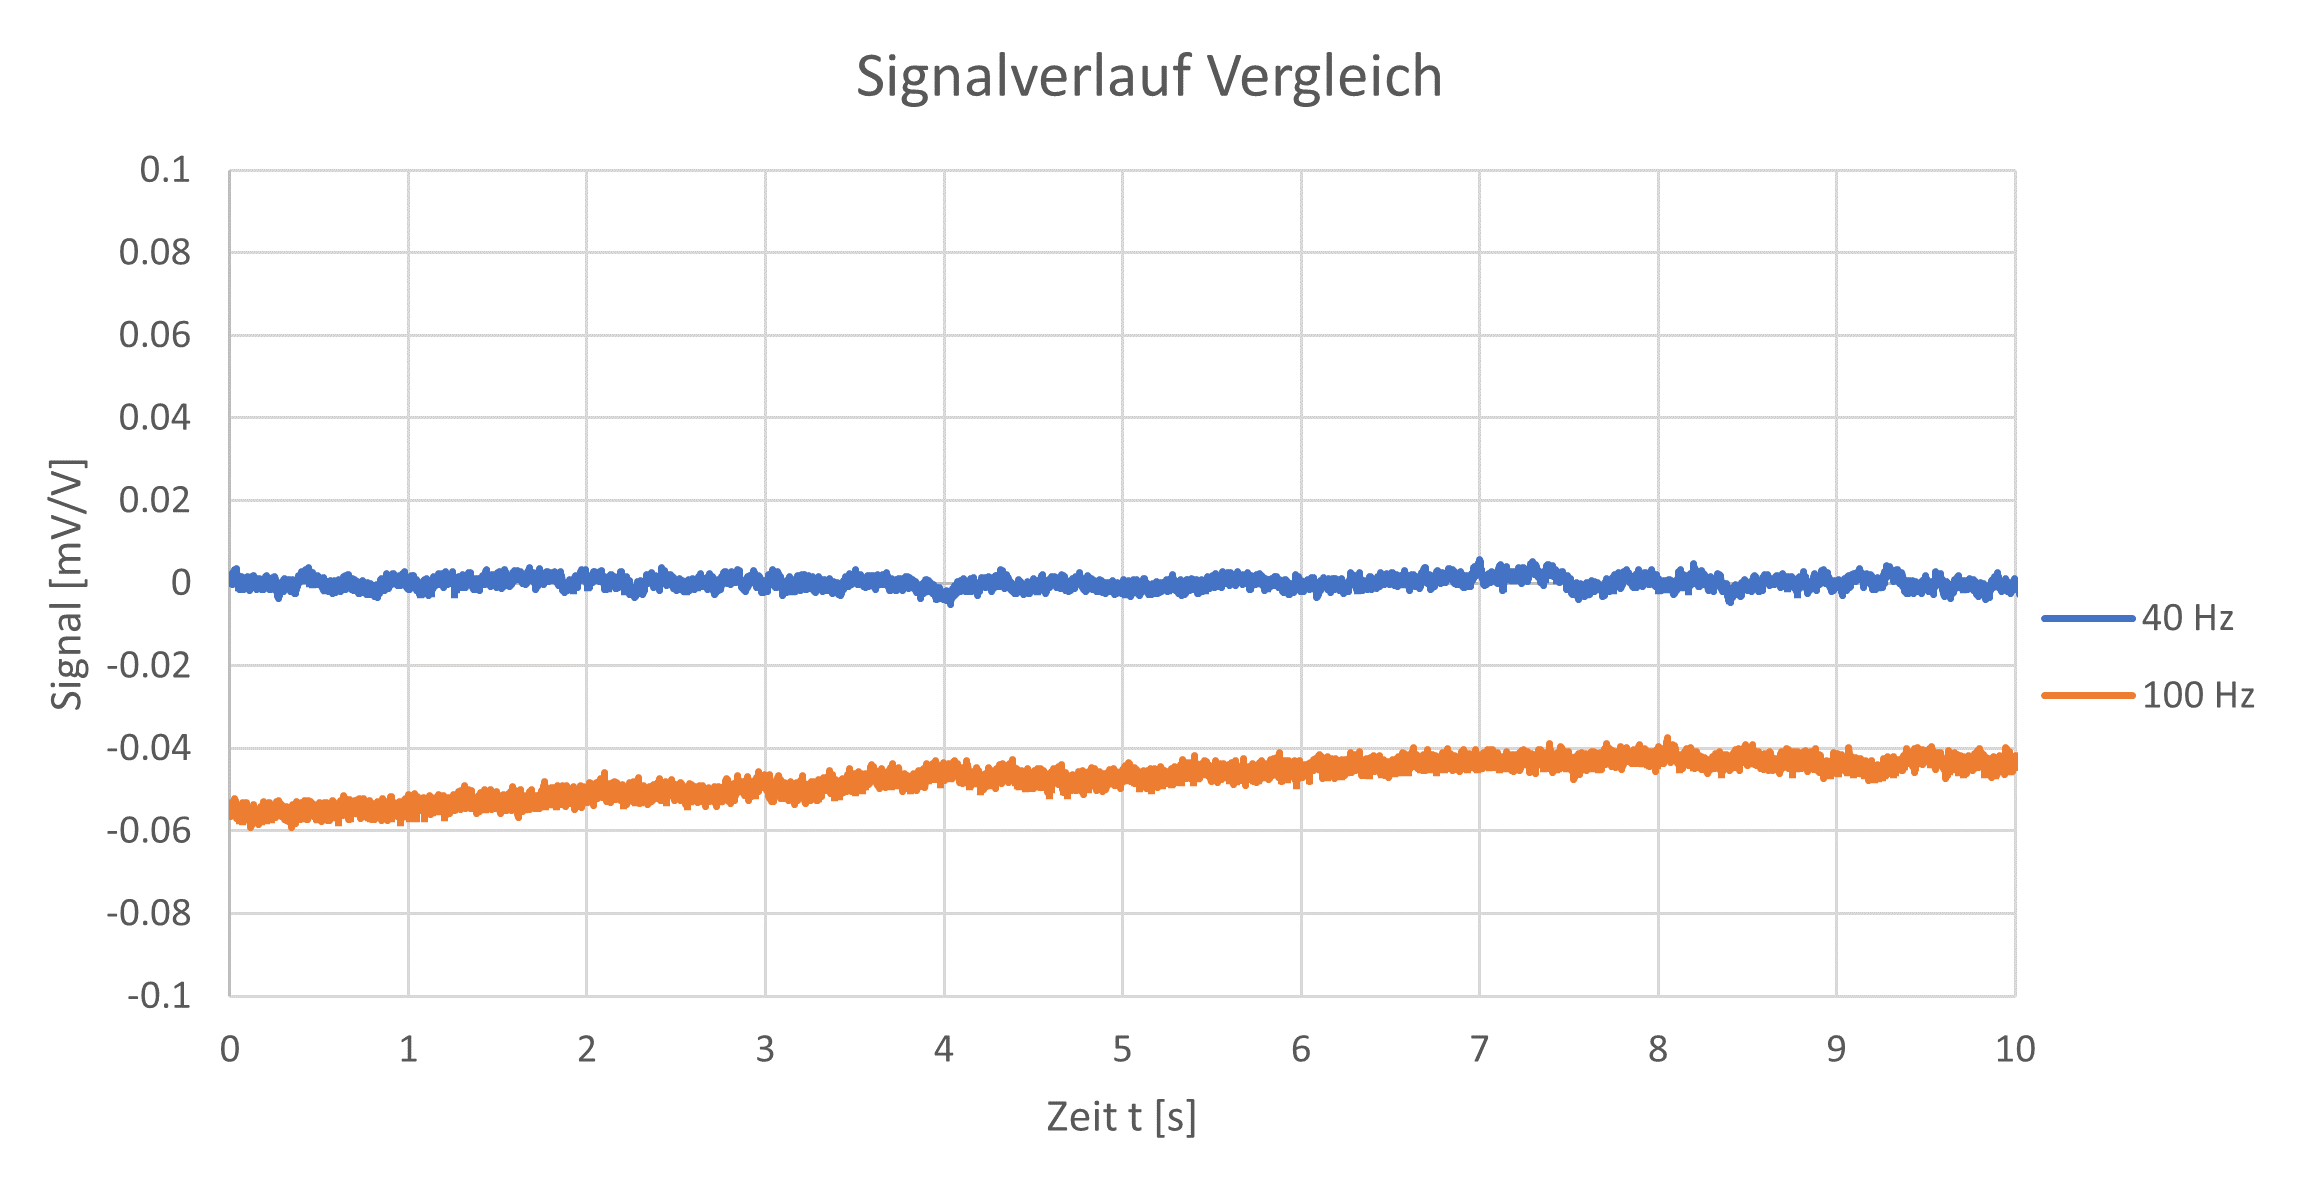
\includegraphics[width=1\linewidth]{imgs/daten_001_NP}
	\caption{Ausschnitt aus Abb. \ref{fig:daten001}; Sensoren unbelastet}
	\label{fig:daten001_NP}
\end{figure}\noindent
Obige Messung wurde ein zweites Mal zur Kontrolle der Reproduzierbarkeit der Phänomene durchgeführt. Die Beobachtungen wurden bestätigt.
\begin{figure}[H]
	\centering
	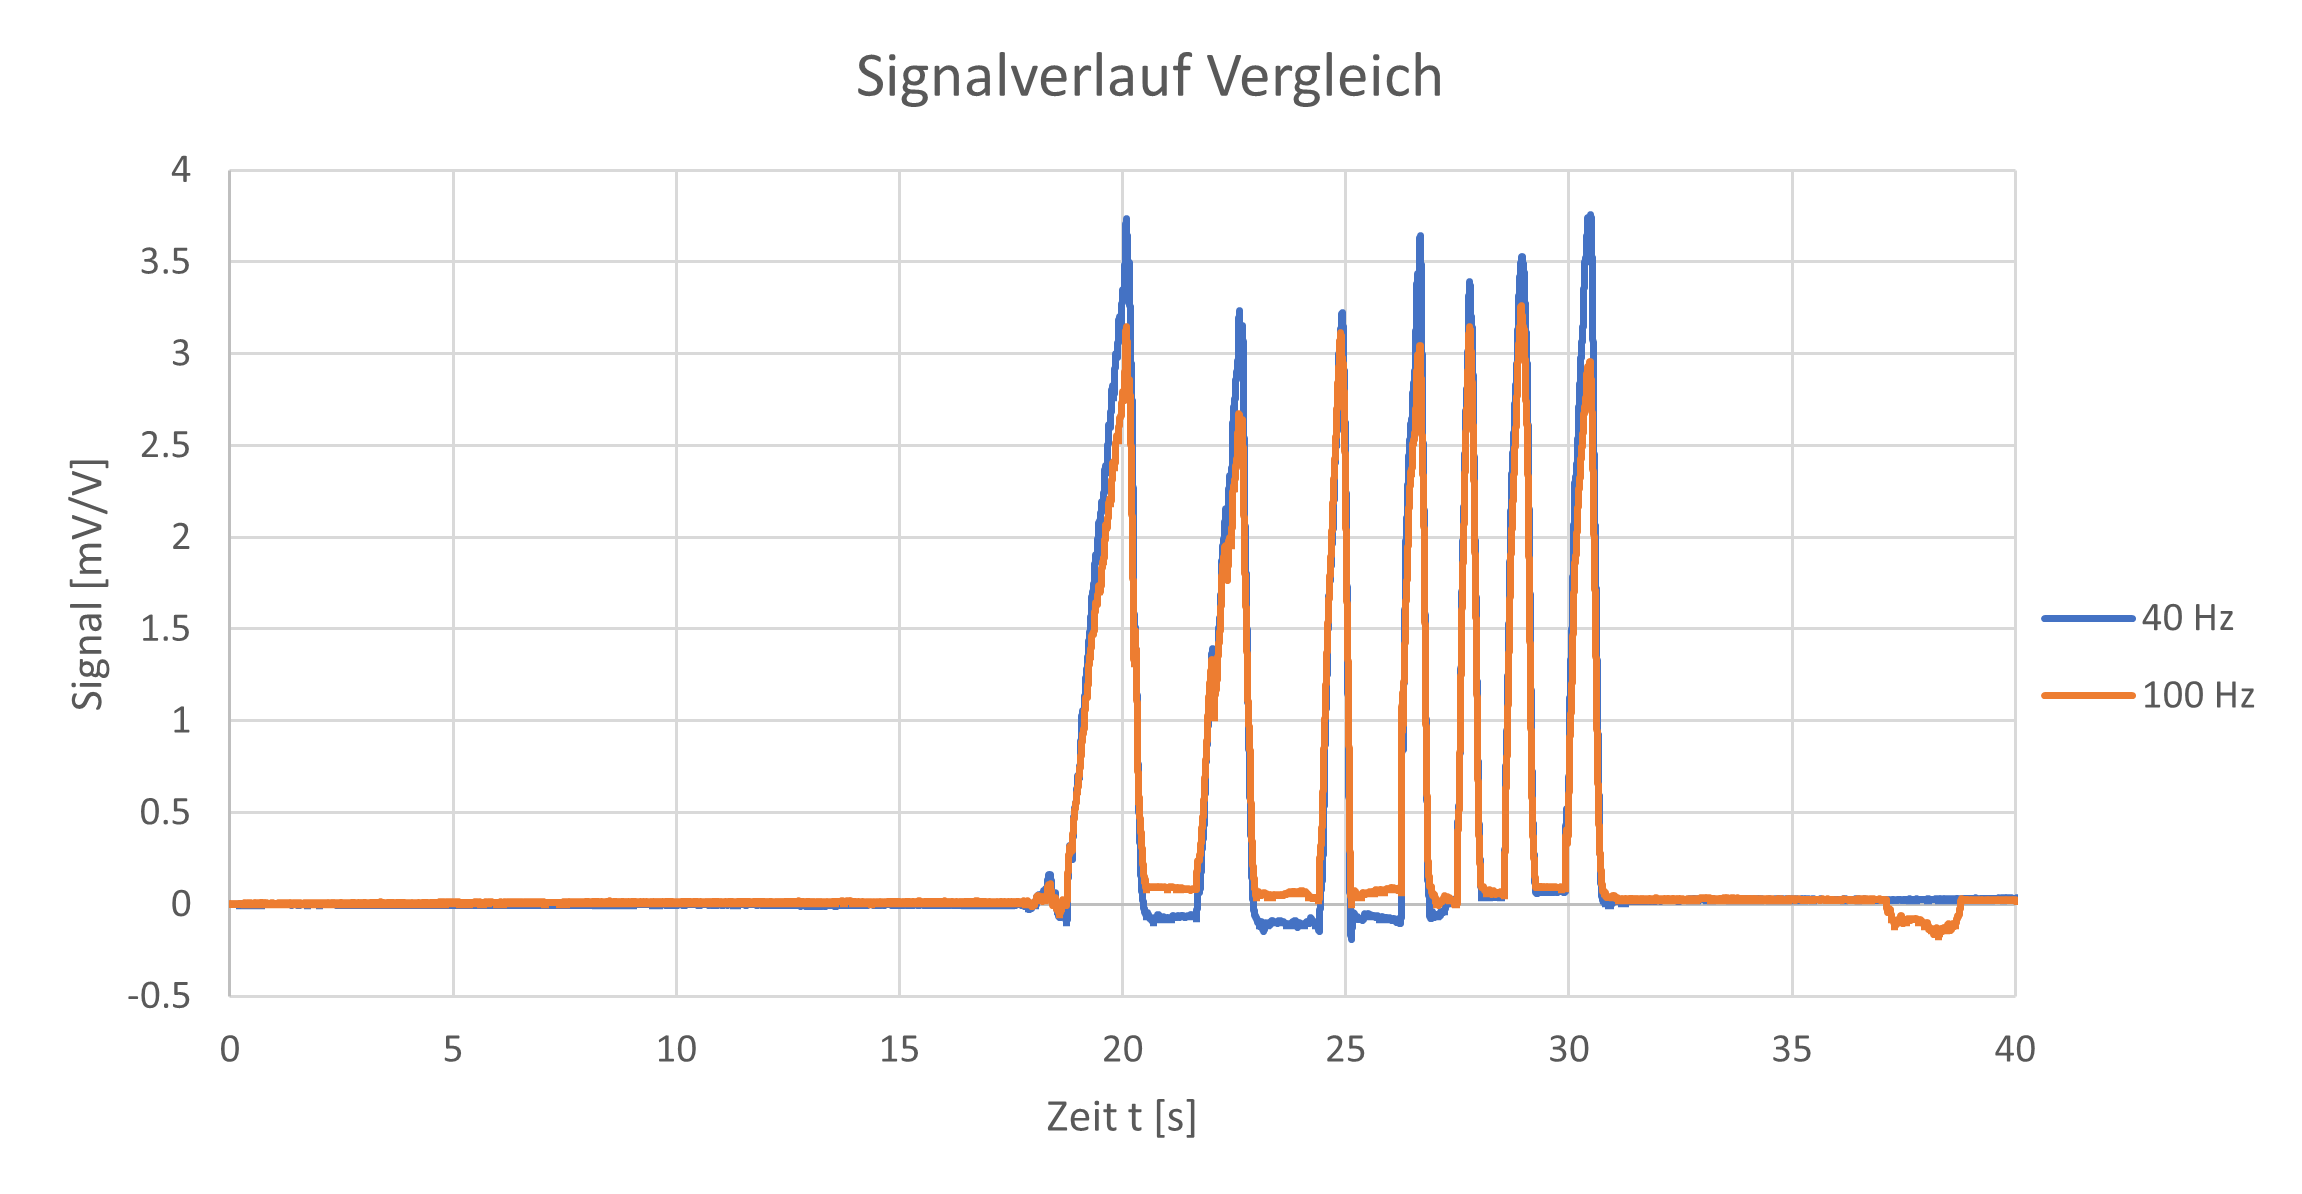
\includegraphics[width=1\linewidth]{imgs/daten_002}
	\caption{Wiederholung der ersten Messung}
	\label{fig:daten002}
\end{figure}
\begin{figure}[H]
	\centering
	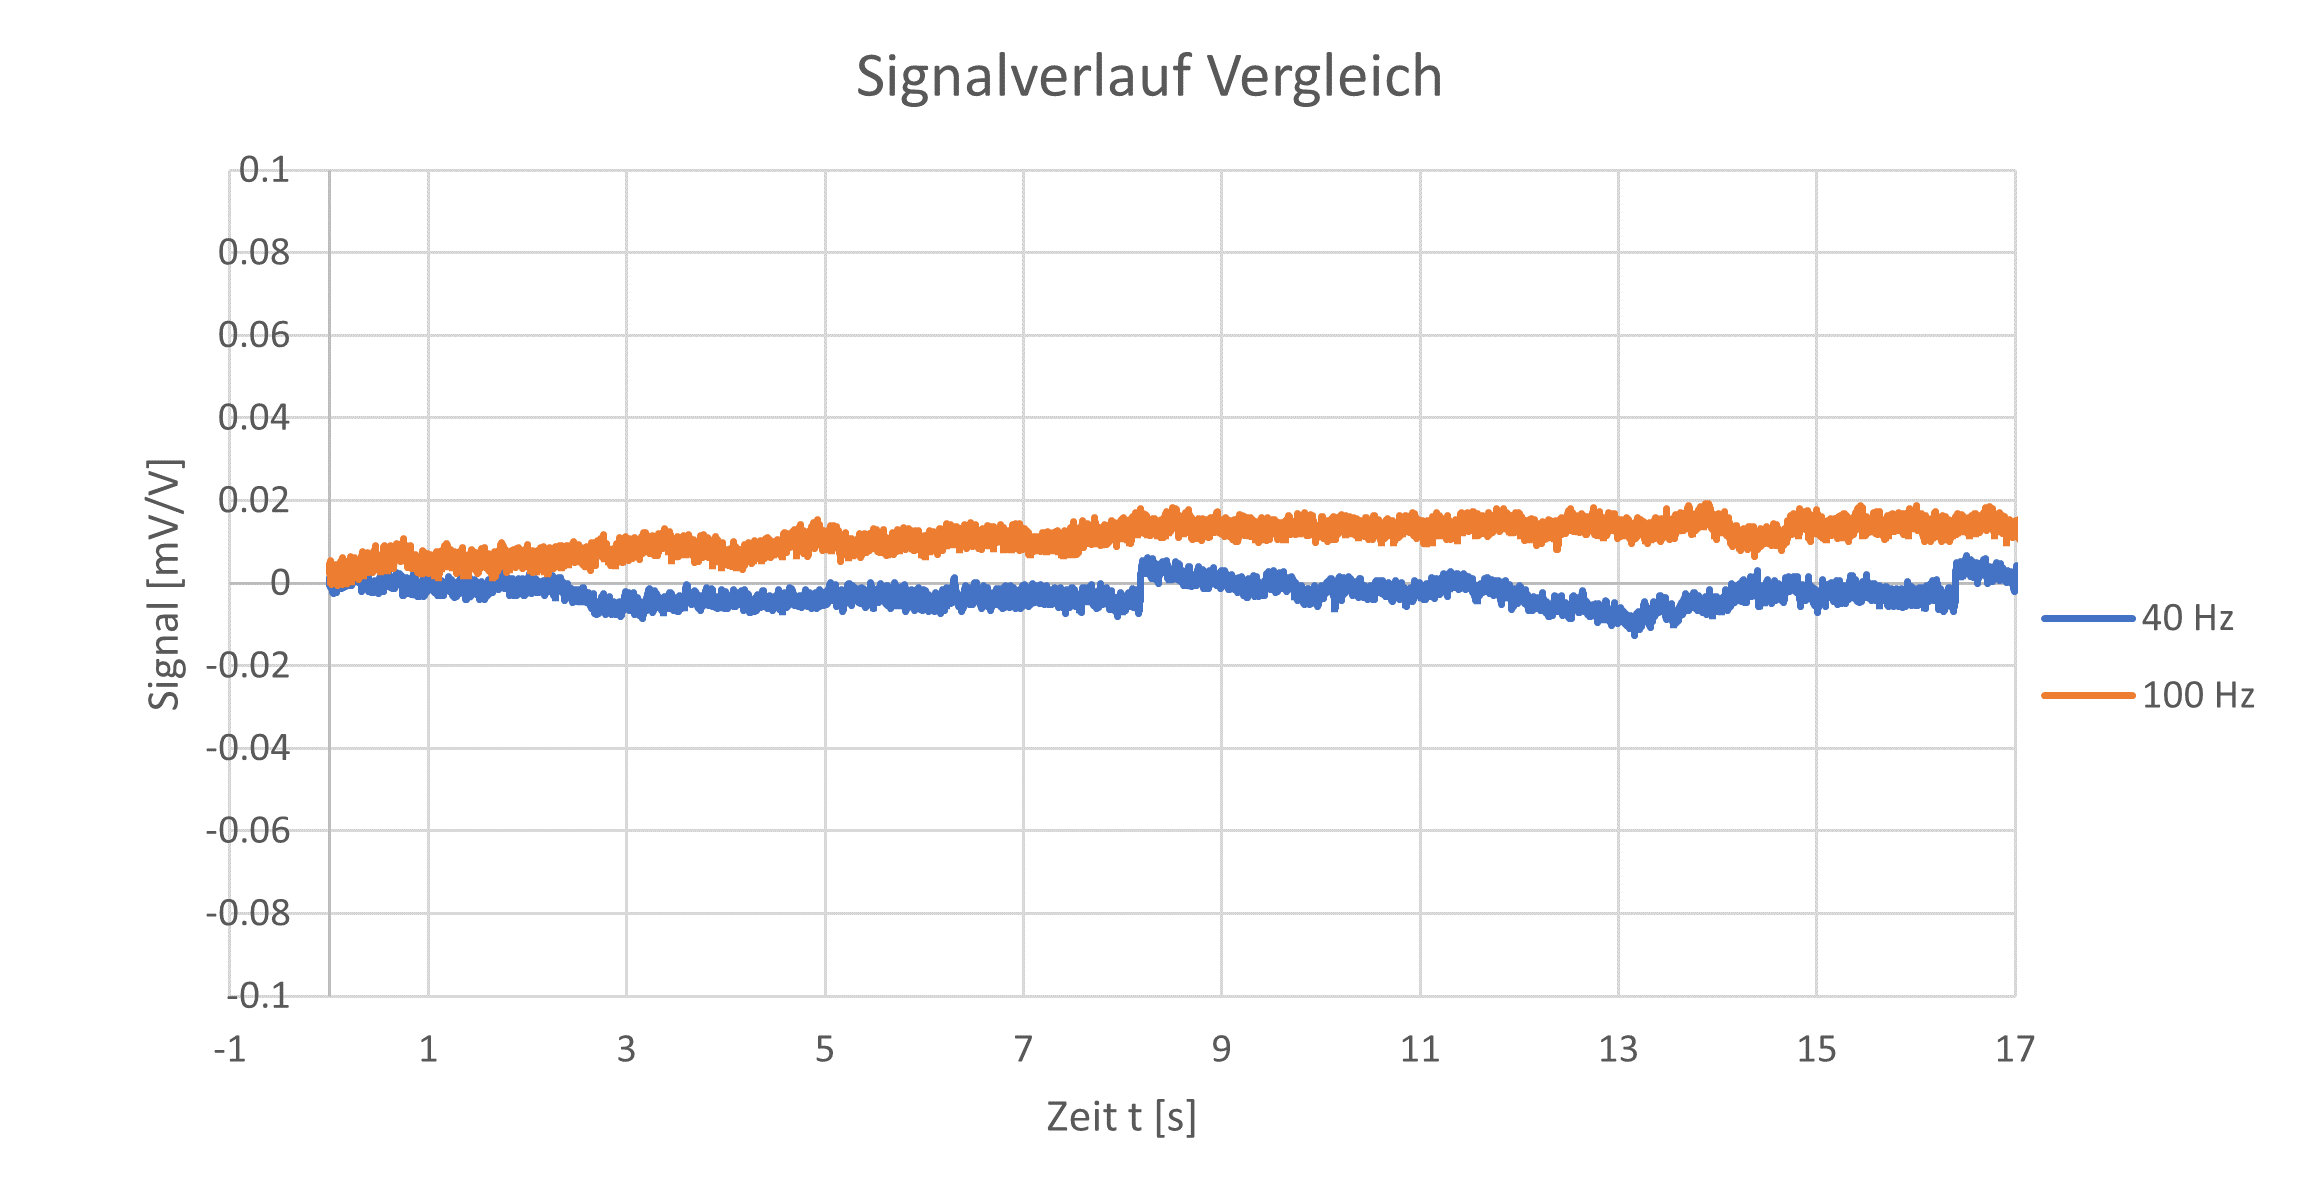
\includegraphics[width=1\linewidth]{imgs/daten_002_NP}
	\caption{Ausschnitt aus Abb. \ref{fig:daten002}; Sensoren unbelastet}
	\label{fig:daten002_NP}
\end{figure}\noindent
Um die Entwicklung der Nullpunktsignals über einen grösseren Zeitraum zu beobachten, wurden die Sensoren über eine Zeitspanne von 30min in unbelastetem Zustand ausgemessen. Die Sensoren sind noch nahezu ''kalt''.
\begin{figure}[H]
	\centering
	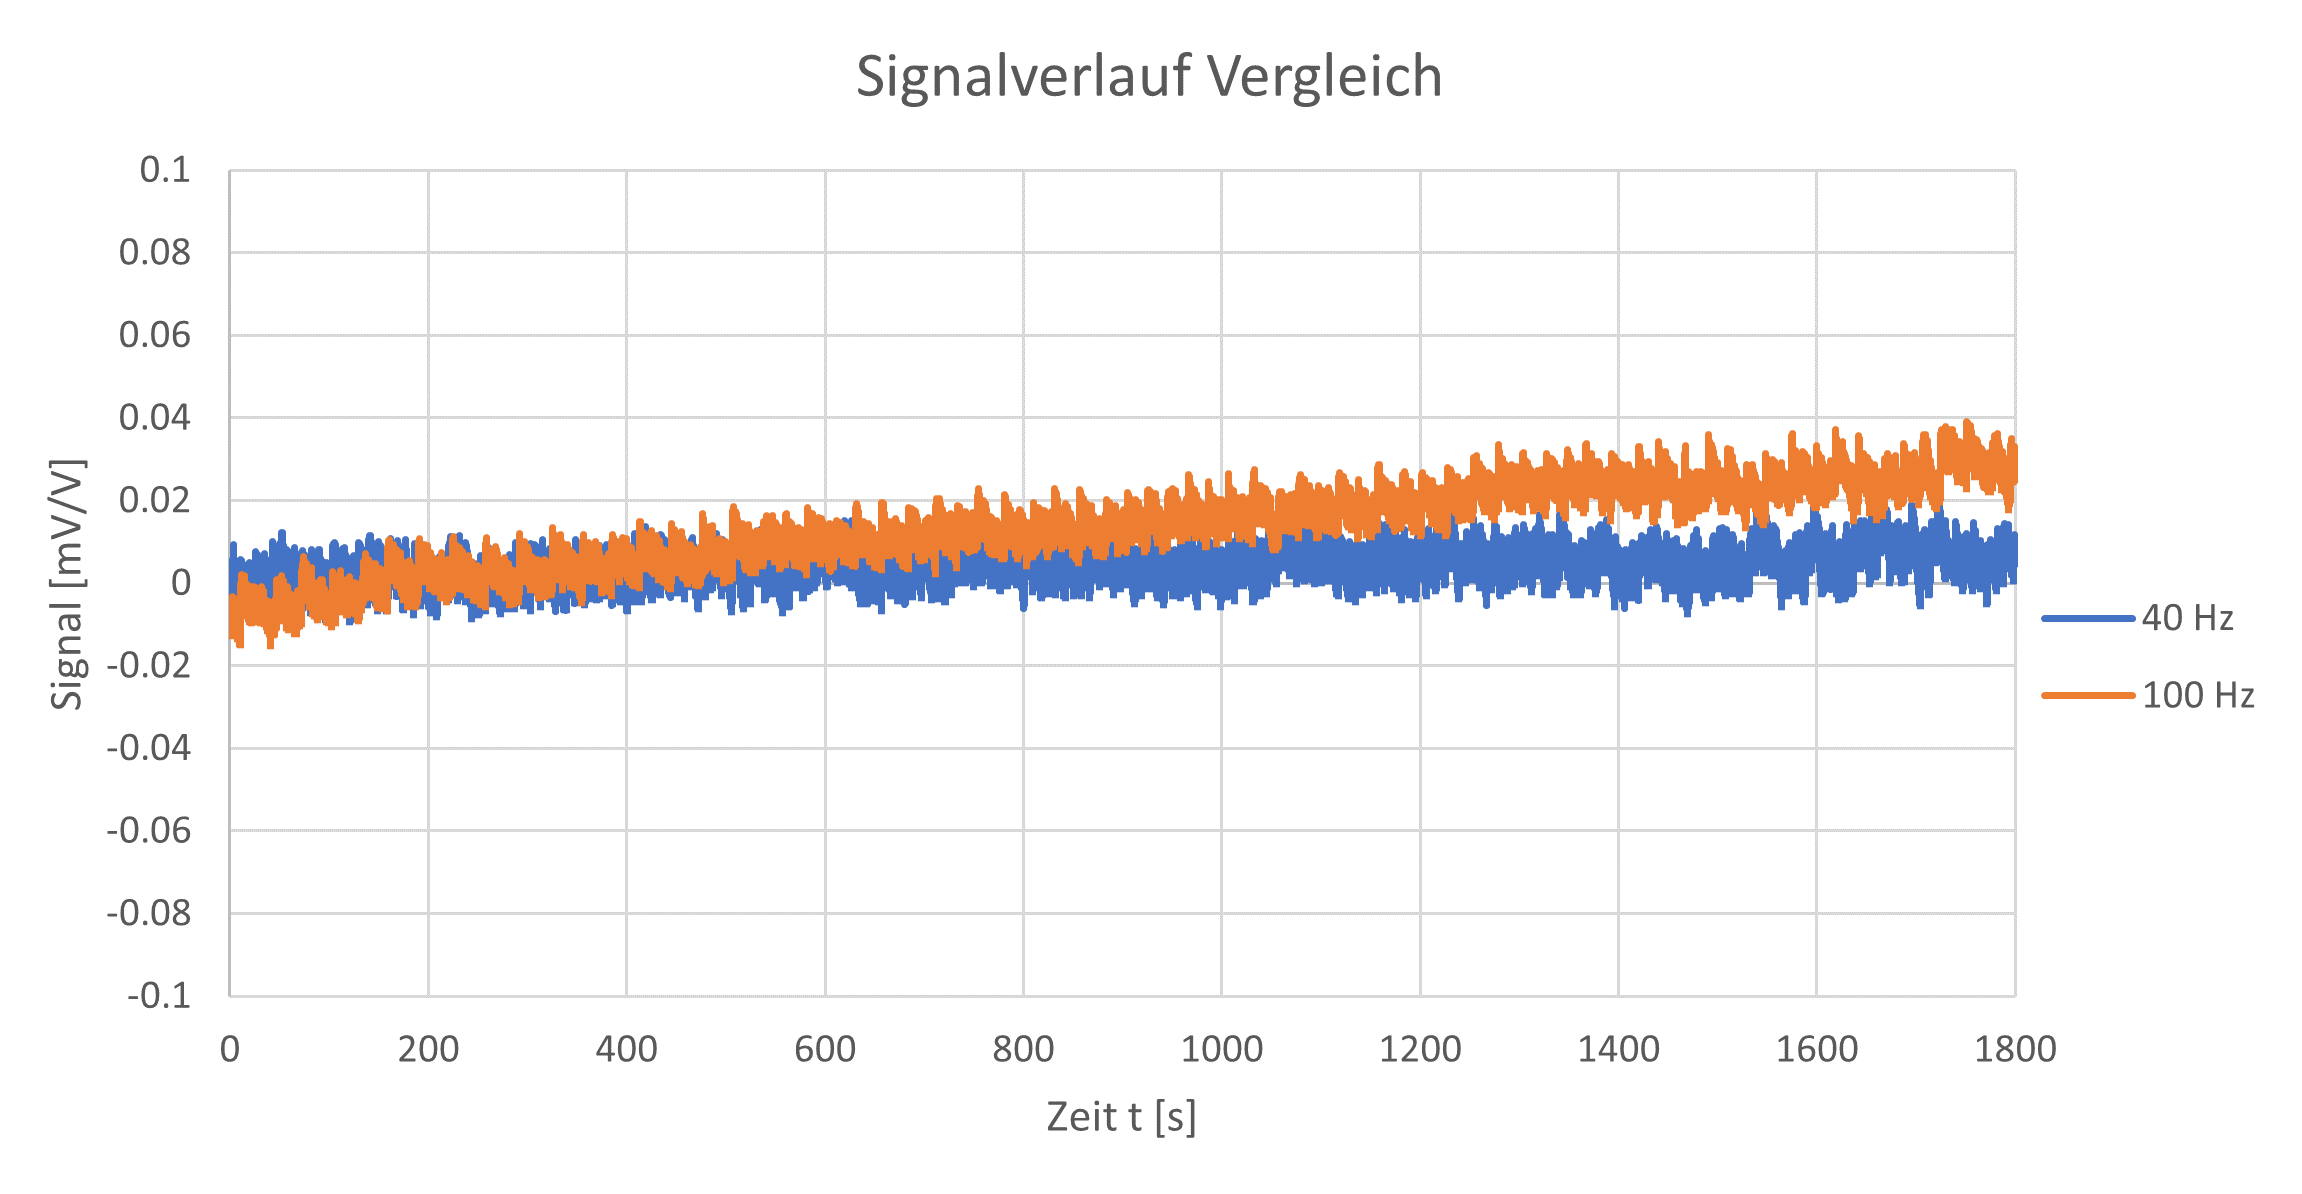
\includegraphics[width=1\linewidth]{imgs/daten_003_kpl}
	\caption{Langzeitbetrachtung Nullpunkt}
	\label{fig:daten003kpl}
\end{figure}
Man erkennt einen deutlichen Drift des Nullpunks des DuT mit EF 100Hz. Dieser driftet um weitere $\sim 30 \mu\varepsilon$, was weiteren $1.5\%$ FS entspricht.
\begin{figure}[H]
	\centering
	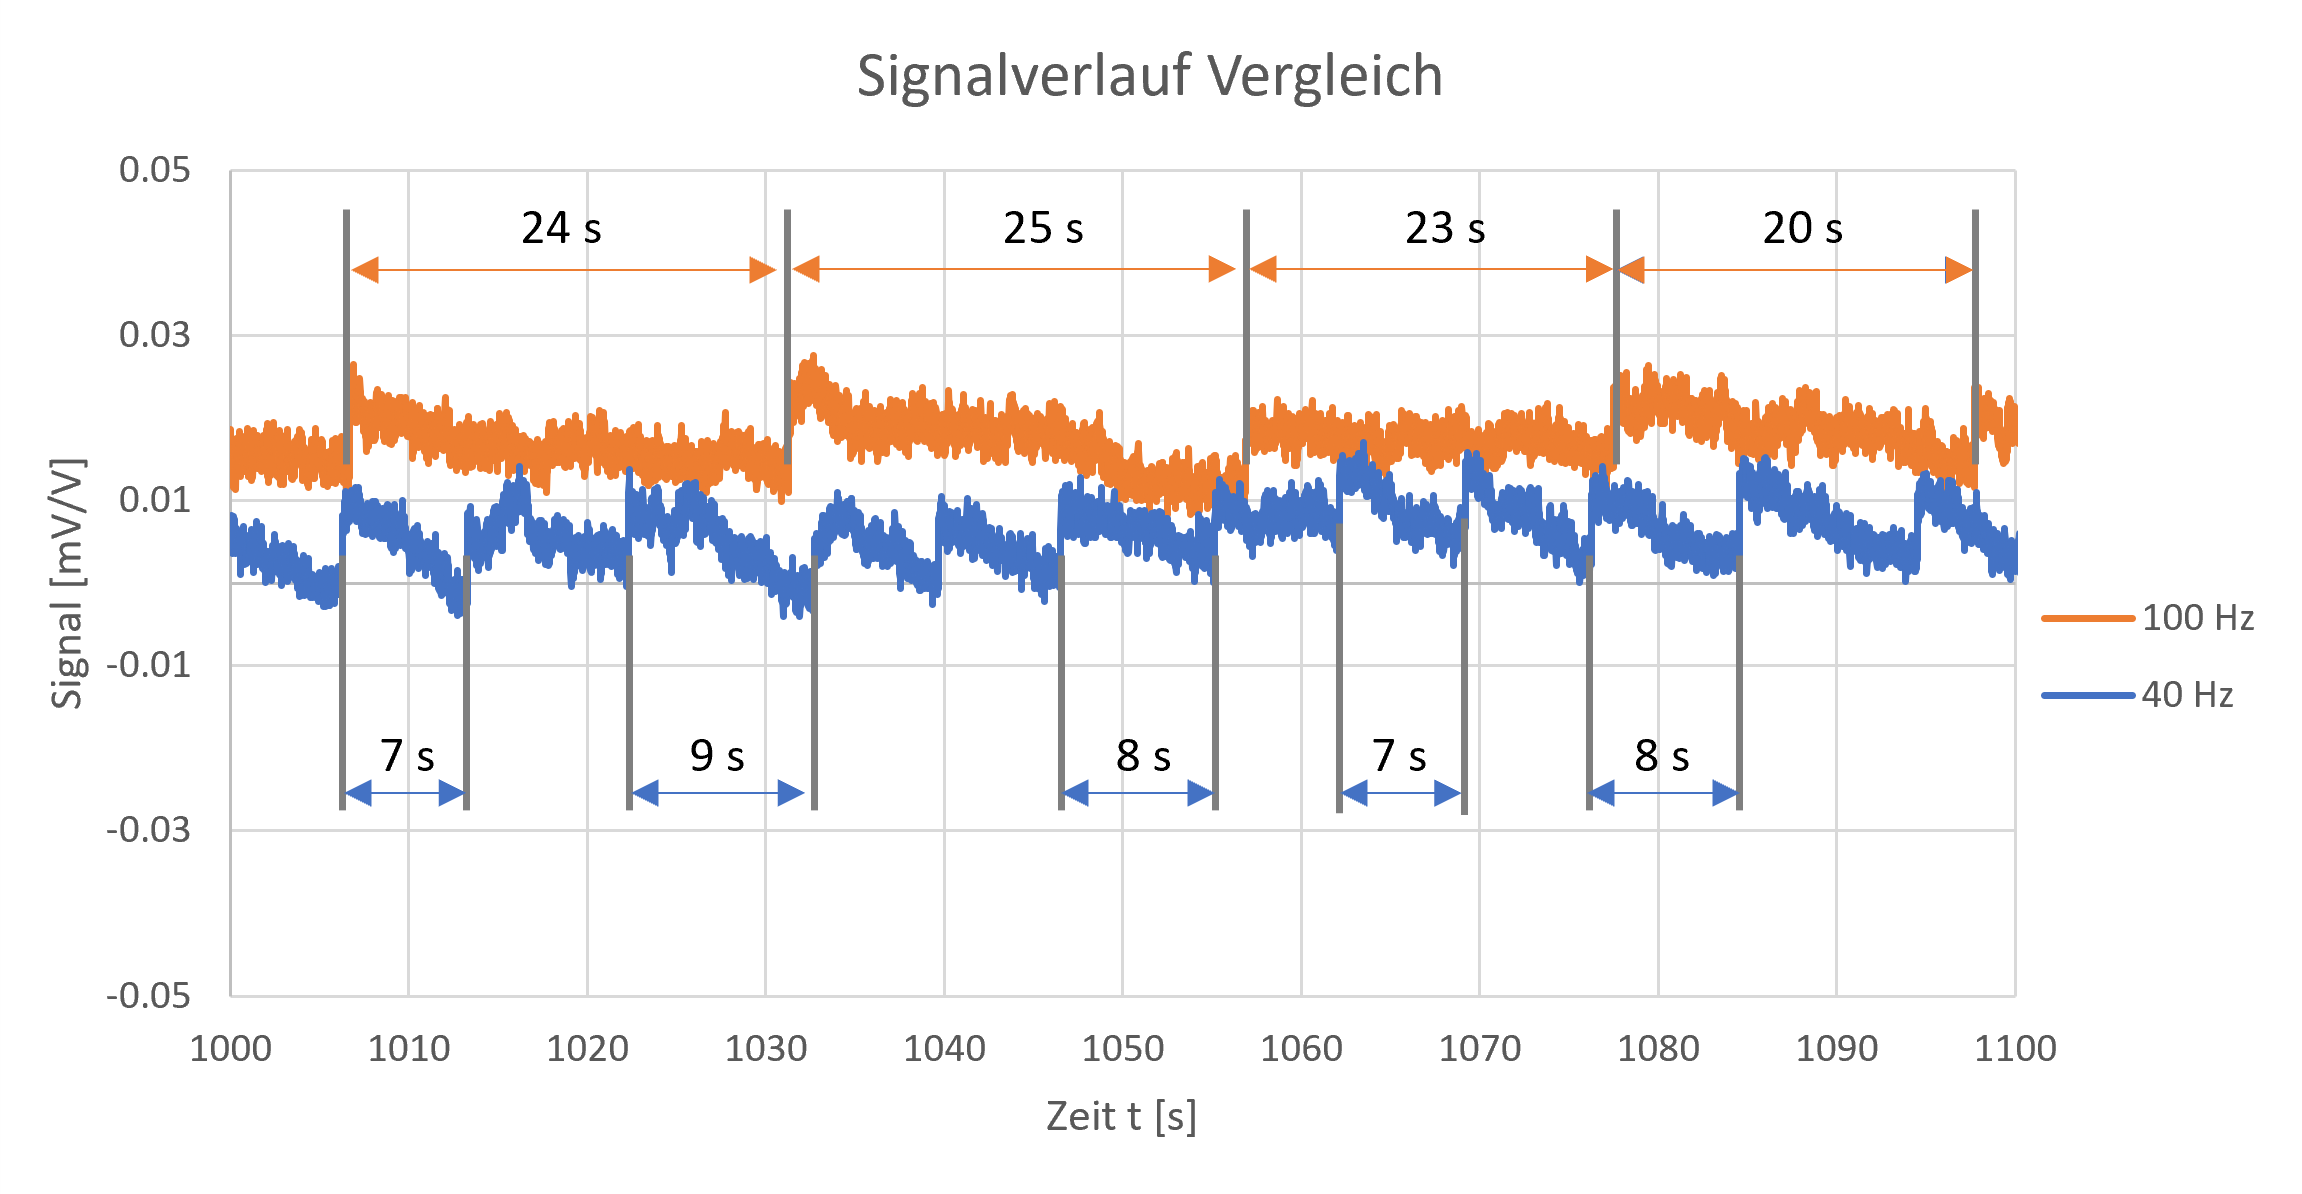
\includegraphics[width=1\linewidth]{imgs/daten_003_detail}
	\caption{Ausschnitt aus Abb. \ref{fig:daten003kpl}: Periodische Sprünge in NP-Signal}
	\label{fig:daten003detail}
\end{figure}\noindent
Wird nun ein Ausschnitt aus obigem Diagramm genauer betrachtet, kann auch hier wieder ein periodisches sprunghaftes Verhalten der Nullpunkte festgestellt werden. Die Periode des DuTs mit EF 40Hz ist wesentlich kürzer als jene des DuTs mit EF 100Hz.
\begin{figure}[H]
	\centering
	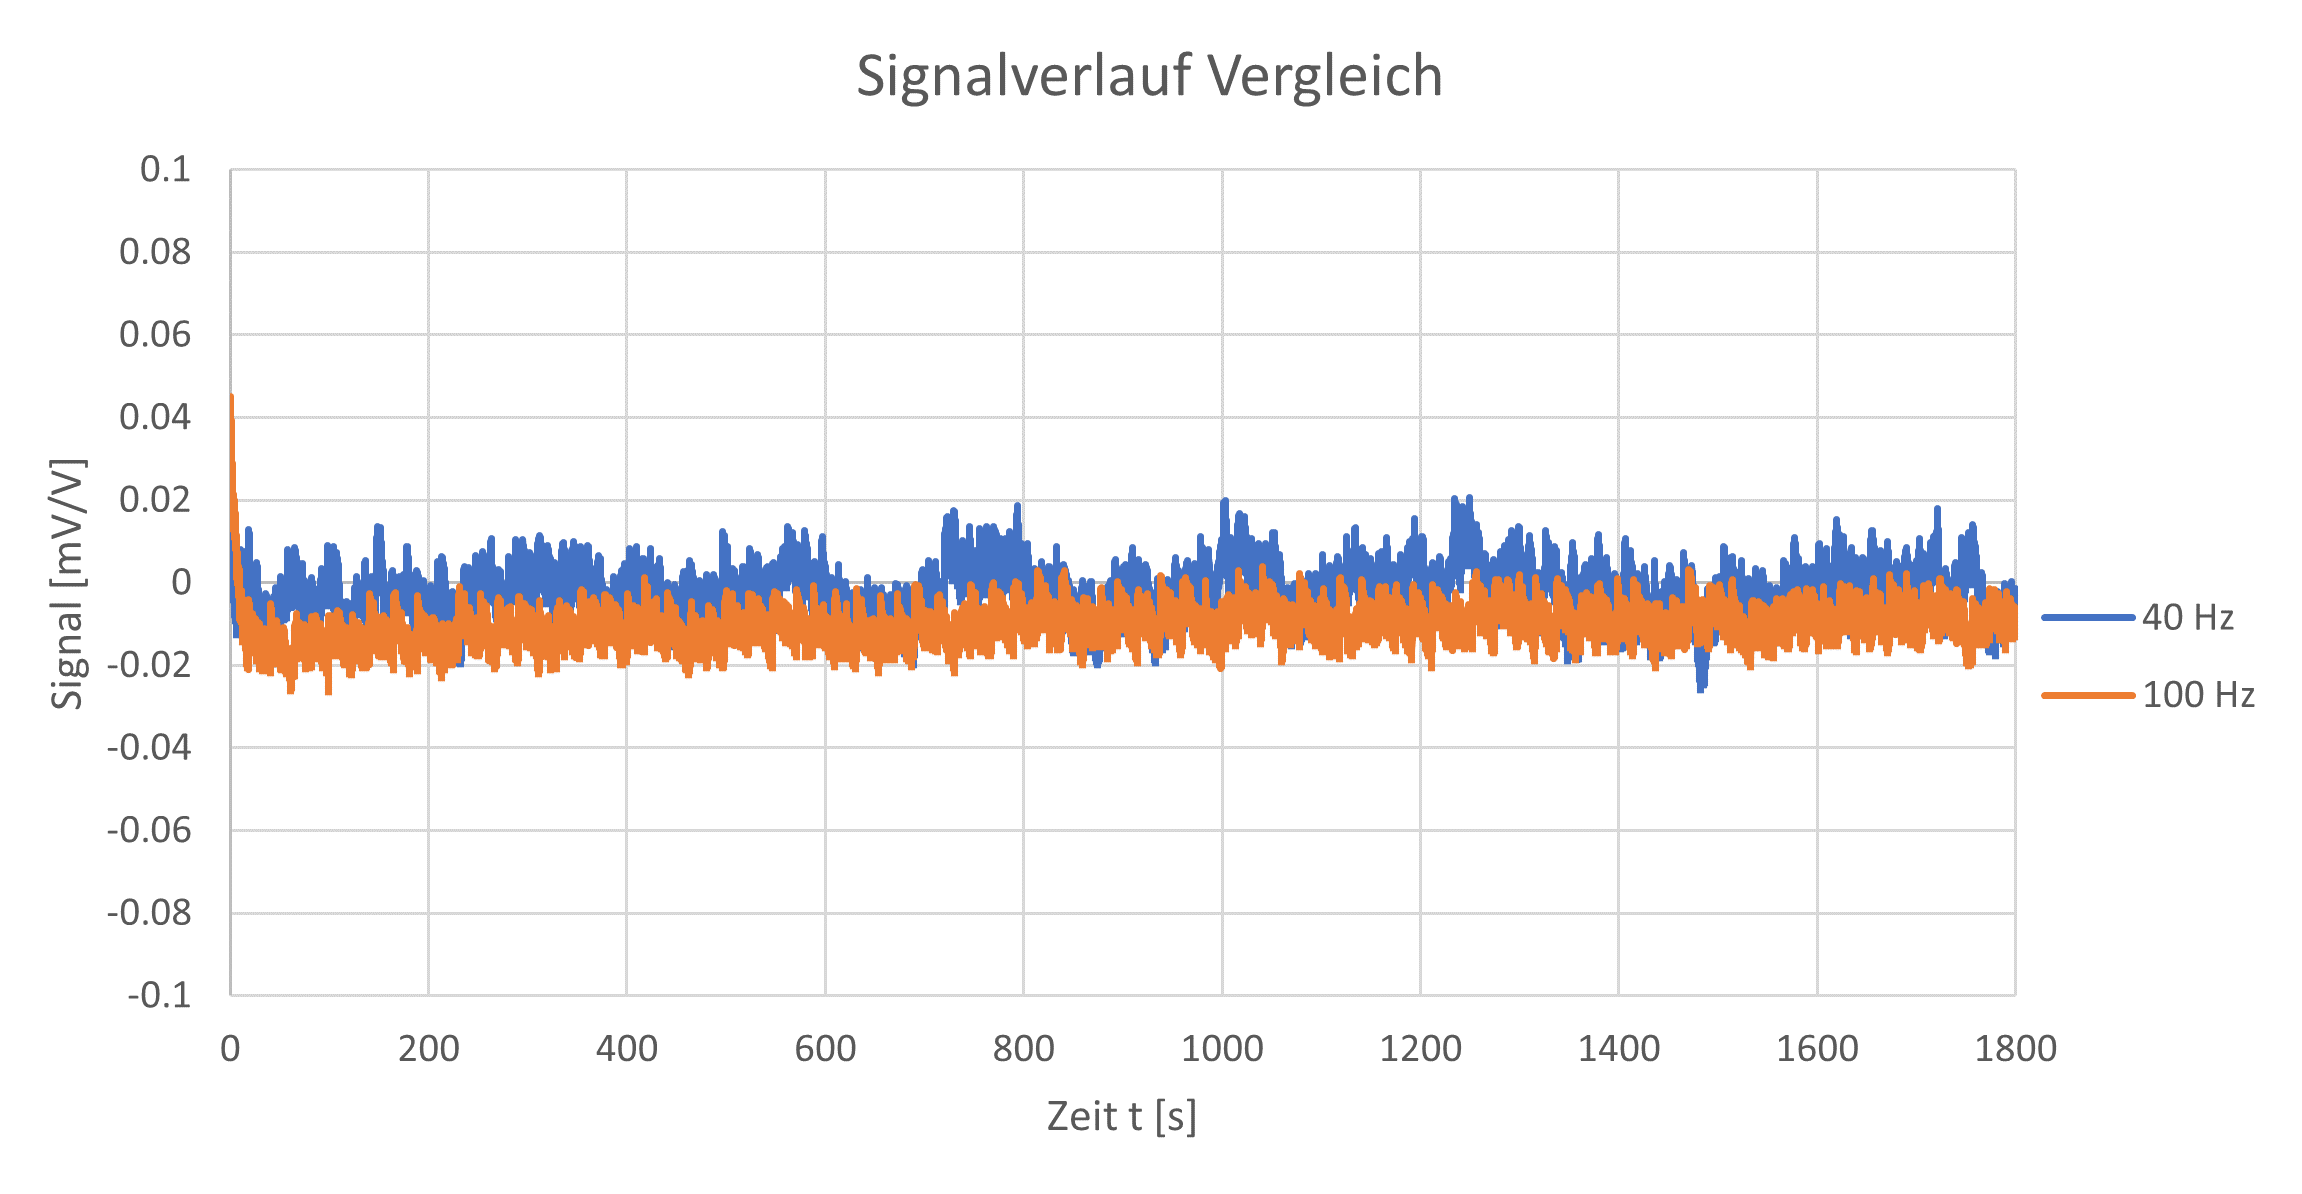
\includegraphics[width=1\linewidth]{imgs/daten_004_kpl}
	\caption{2. Langzeitbetrachtung Nullpunkt (Sensoren warmgelaufen)}
	\label{fig:daten004kpl}
\end{figure}\noindent
Obige Messung wurde nach rund 1h wiederholt. Die Sensoren wurden durchgehend bestromt und sind zum Start dieser Messung deutlich wärmer als zu Beginn.
\begin{figure}[H]
	\centering
	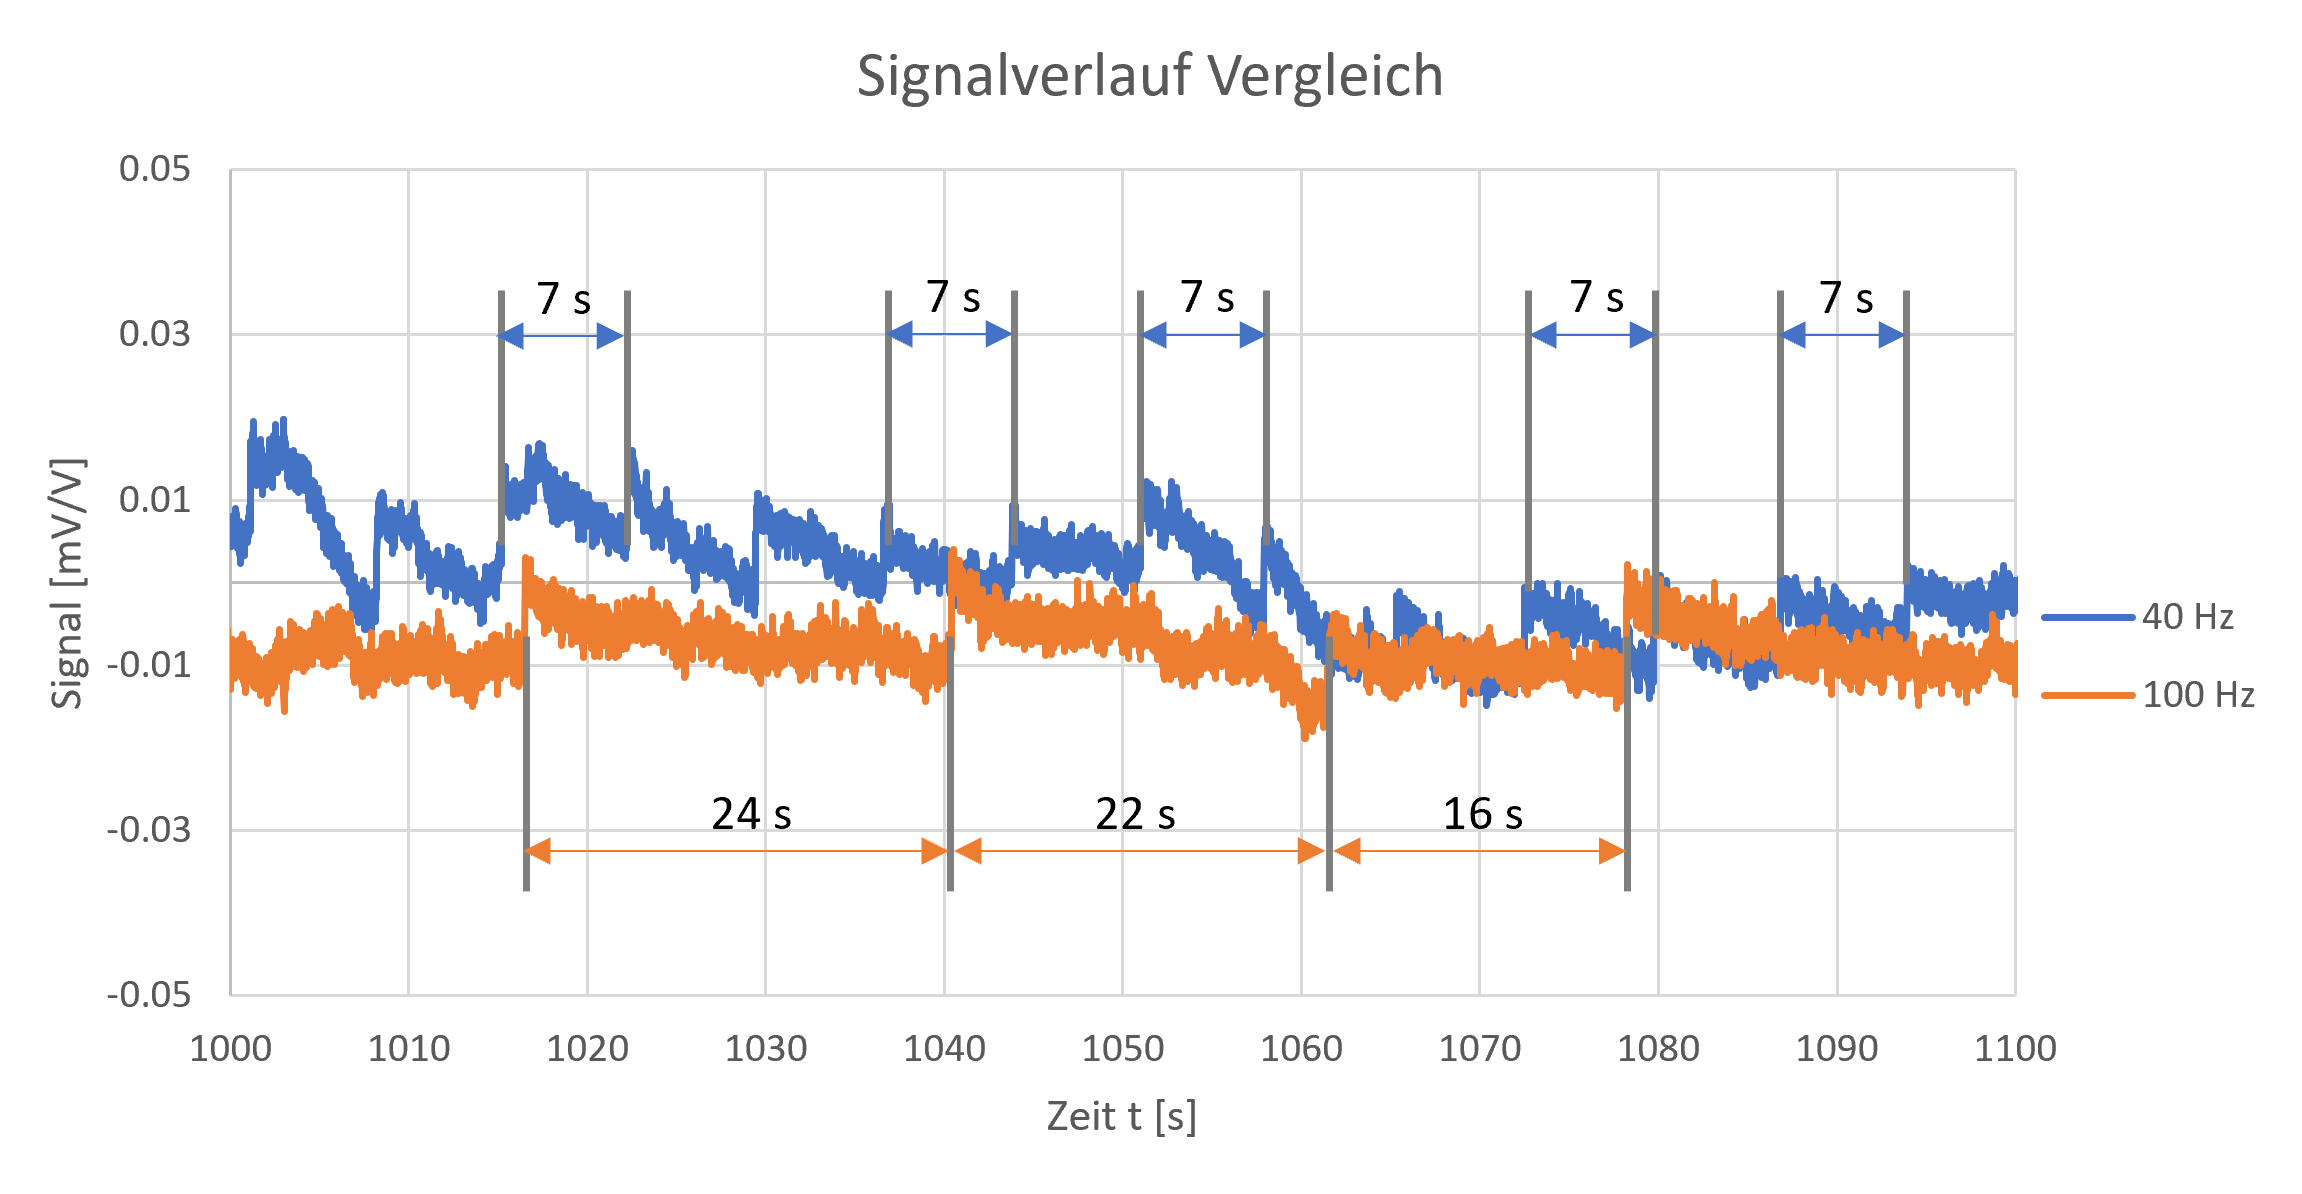
\includegraphics[width=1\linewidth]{imgs/daten_004_detail}
	\caption{Ausschnitt aus Abb. \ref{fig:daten004kpl}: Periodische Sprünge in NP-Signal}
	\label{fig:daten004detail}
\end{figure}\noindent
Insgesamt kann keine merkliche Veränderung gegenüber der Messung im ''kalten'' Zustand festgestellt werden. Es ist jedoch zu beobachten, dass der Nullpunkt des DuTs mit EF 100Hz gleich zu Beginn der Messung abfällt. Bei der ersten Messung konnte ein klarer Trend für eine Zunahme des NP-Signals festgestellt werden. Auch über den Zeitraum von weiteren 30min scheint der NP nun bei beiden DuTs stabil zu sein. Das sprunghafte Verhalten kann aber weiterhin beobachtet werden, wie der Ausschnitt in \ref{fig:daten004detail} zeigt.\\
Zum Schnuss wurde die aller erste Messung nochmal wiederholt, um Temperatureinflüsse (beide Sensoren nun in steady state, Temperatur ''Handwarm'') zu untersuchen. Die Charakteristik der Verläufe blieb aber unverändert, wie der Abbildung \ref{fig:daten006kpl} zu entnehmen ist. 
\begin{figure}[H]
	\centering
	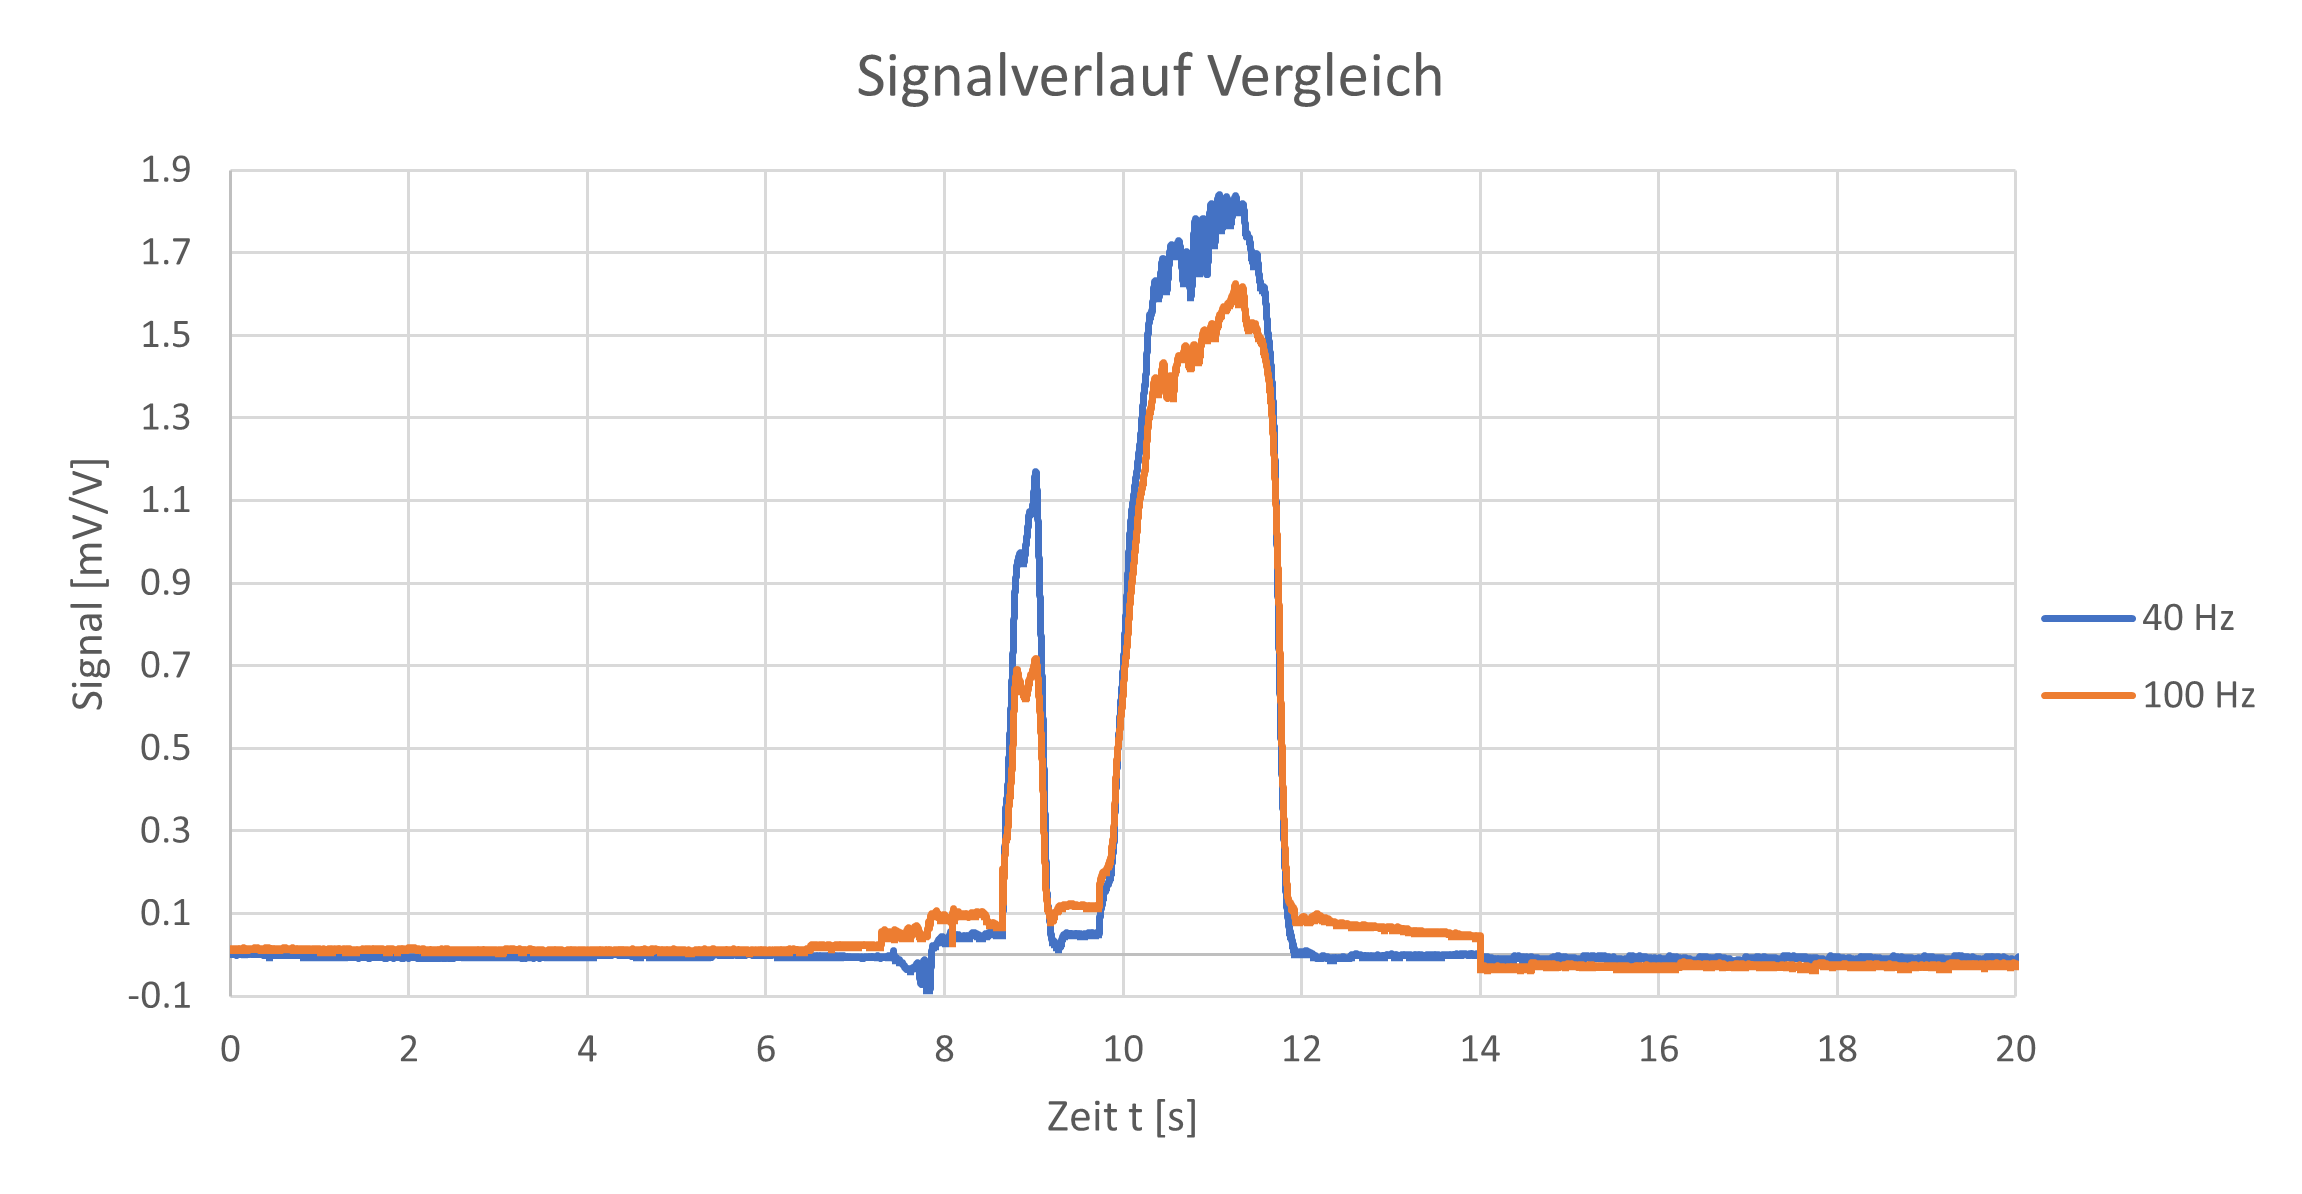
\includegraphics[width=1\linewidth]{imgs/daten_006_kpl}
	\caption{40 Hz (unvergossen) vs 100 Hz (vergossen) bei vergleichbarer Belastung; beide Sensoren ''warmgelaufen''}
	\label{fig:daten006kpl}
\end{figure}\noindent
\section{Vergleich DuT 500Hz (unvergossen) vs DuT 20Hz (unvergossen)}
Die beiden Messungen (Langzeit-NP-Betrachtung, ''Rücken an Rücken''-Belastung) wurde mit den DuTs mit EF 500Hz und EF 20Hz widerholt. Die Resultate  sind den folgenden 3 Abbildungen zu entnehmen. Insgesamt kann festgestellt werden, dass der NP dieser beiden DuTs stabil zu sein scheinen, relativ symmetrisch um 0 sind und keine deutlichen Sprünge respektive keine deutliche Periodizität aufweisen. \\
Das Nullpunktverhalten bei punktueller Belastung ist ebenfalls mit jenem der vorangegangenen DuTs vergleichbar.
\begin{figure}[H]
	\centering
	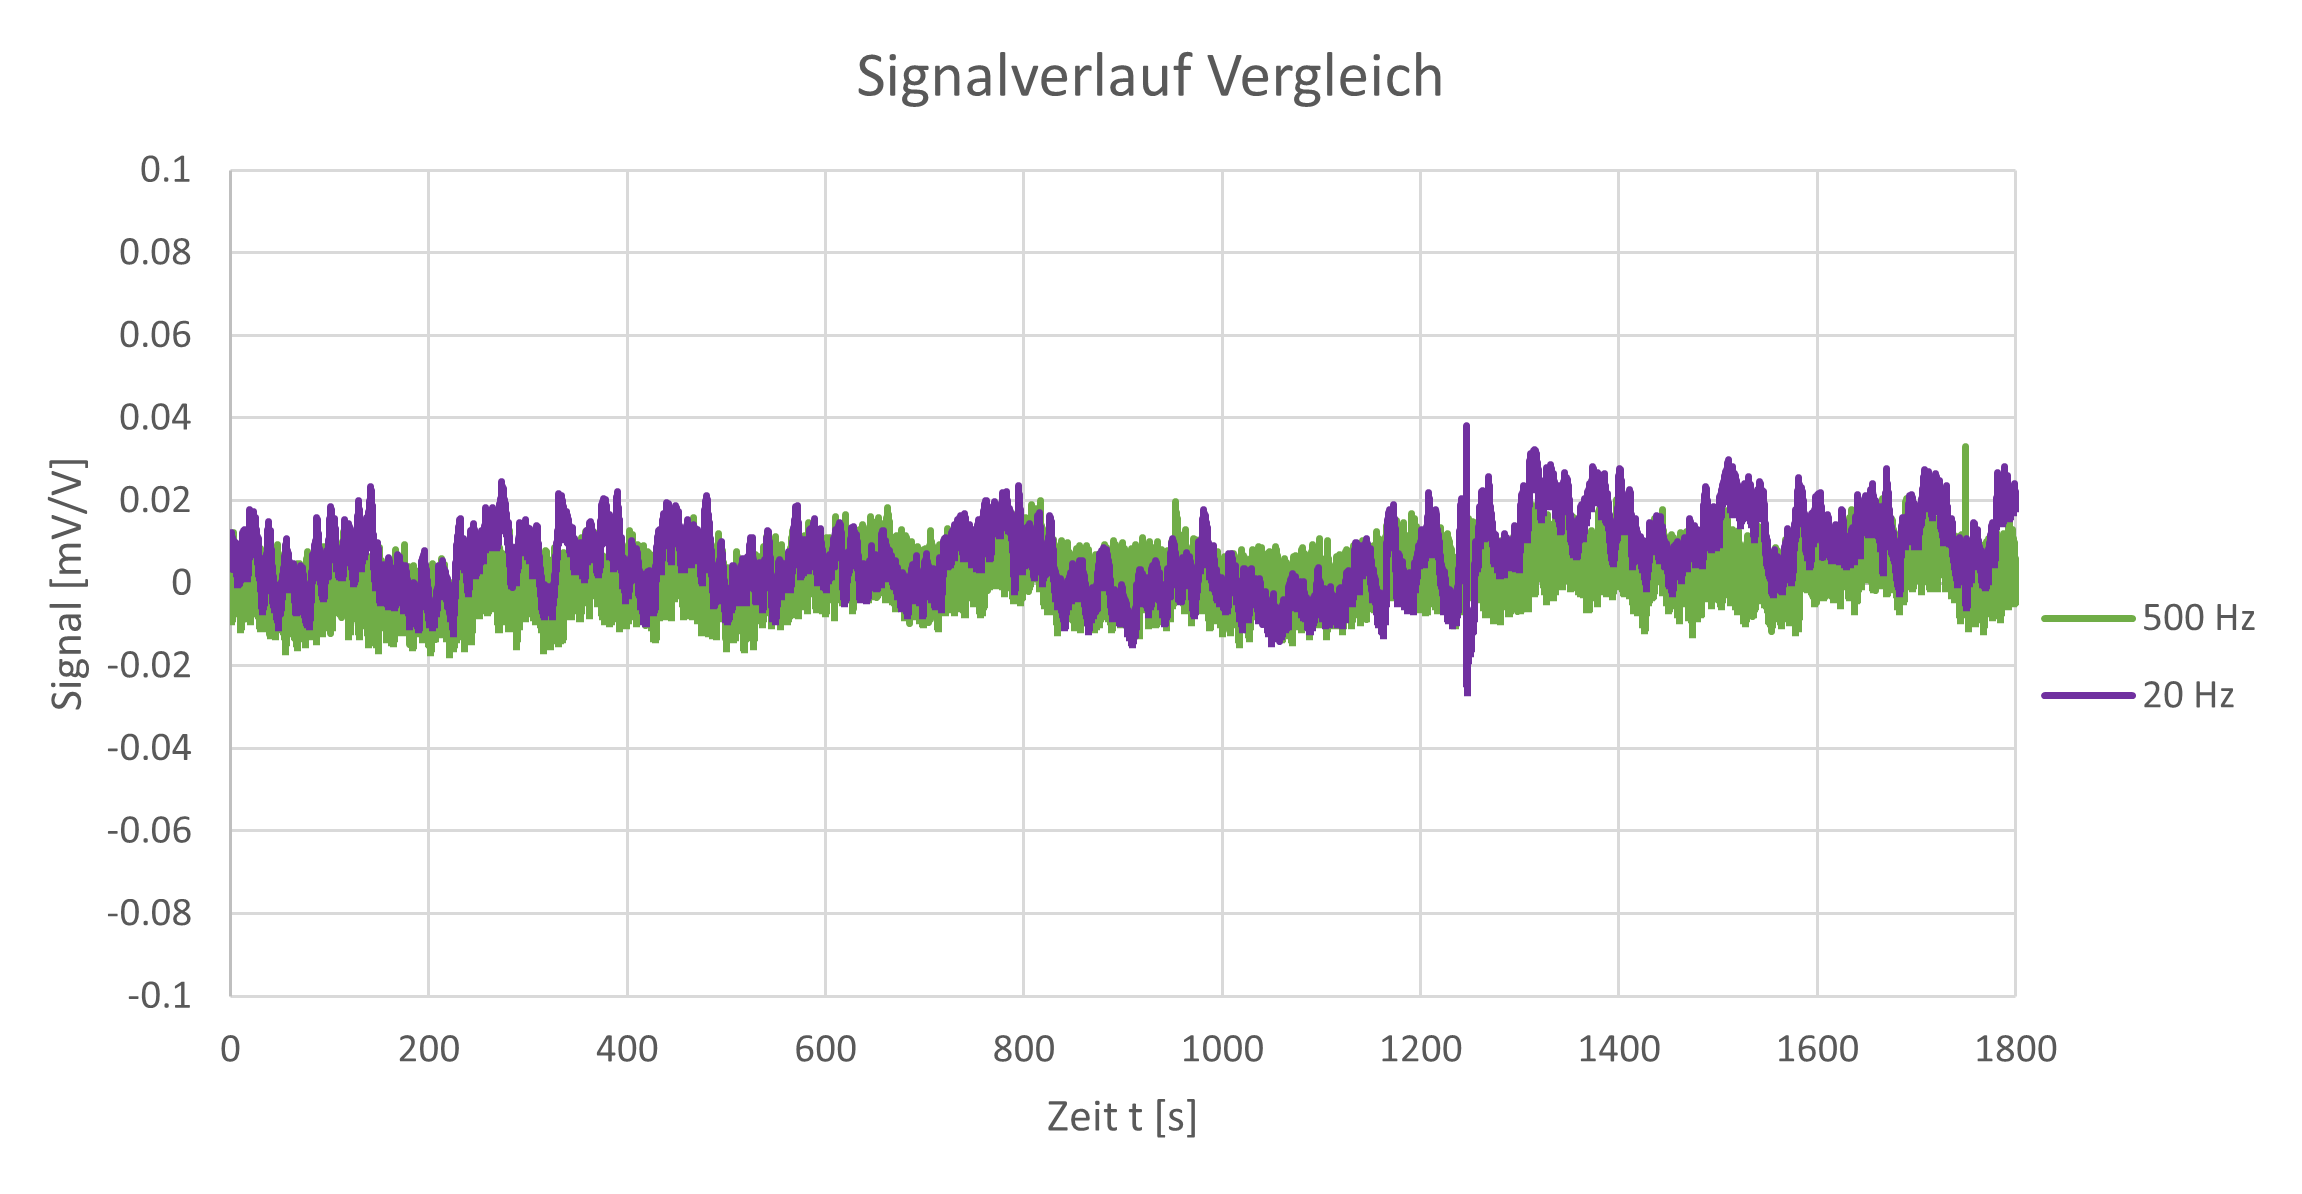
\includegraphics[width=1\linewidth]{imgs/daten_007_kpl}
	\caption{Langzeitbetrachtung Nullpunkt DuTs 500 Hz und 20 Hz}
	\label{fig:daten007kpl}
\end{figure}
\begin{figure}[H]
	\centering
	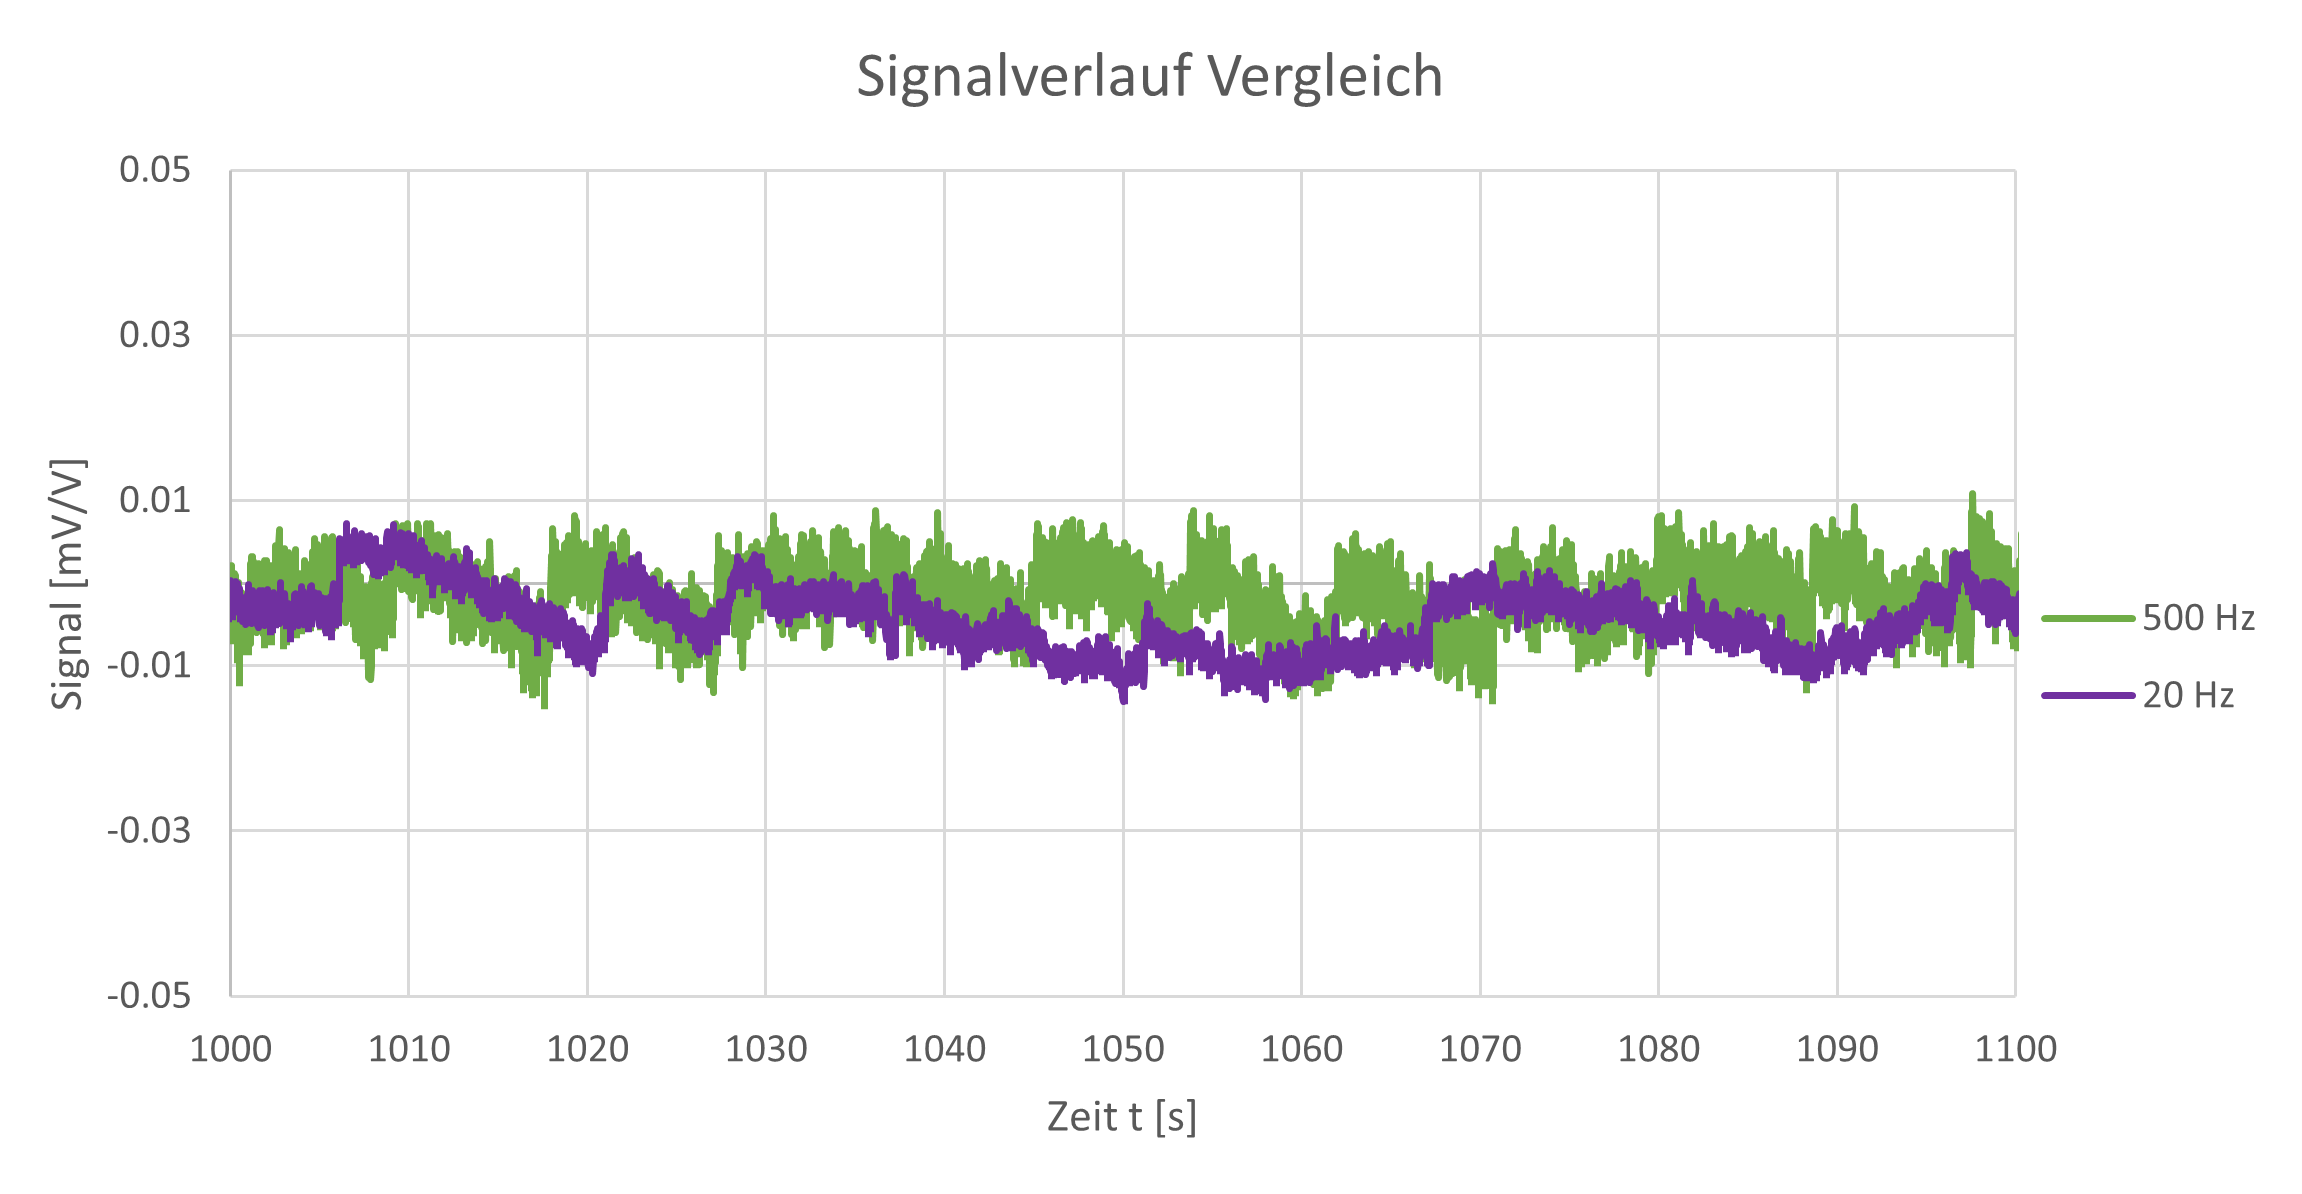
\includegraphics[width=1\linewidth]{imgs/daten_007_detail}
	\caption{Ausschnitt aus Abb. \ref{fig:daten007kpl}}
	\label{fig:daten007detail}
\end{figure}
\begin{figure}[H]
	\centering
	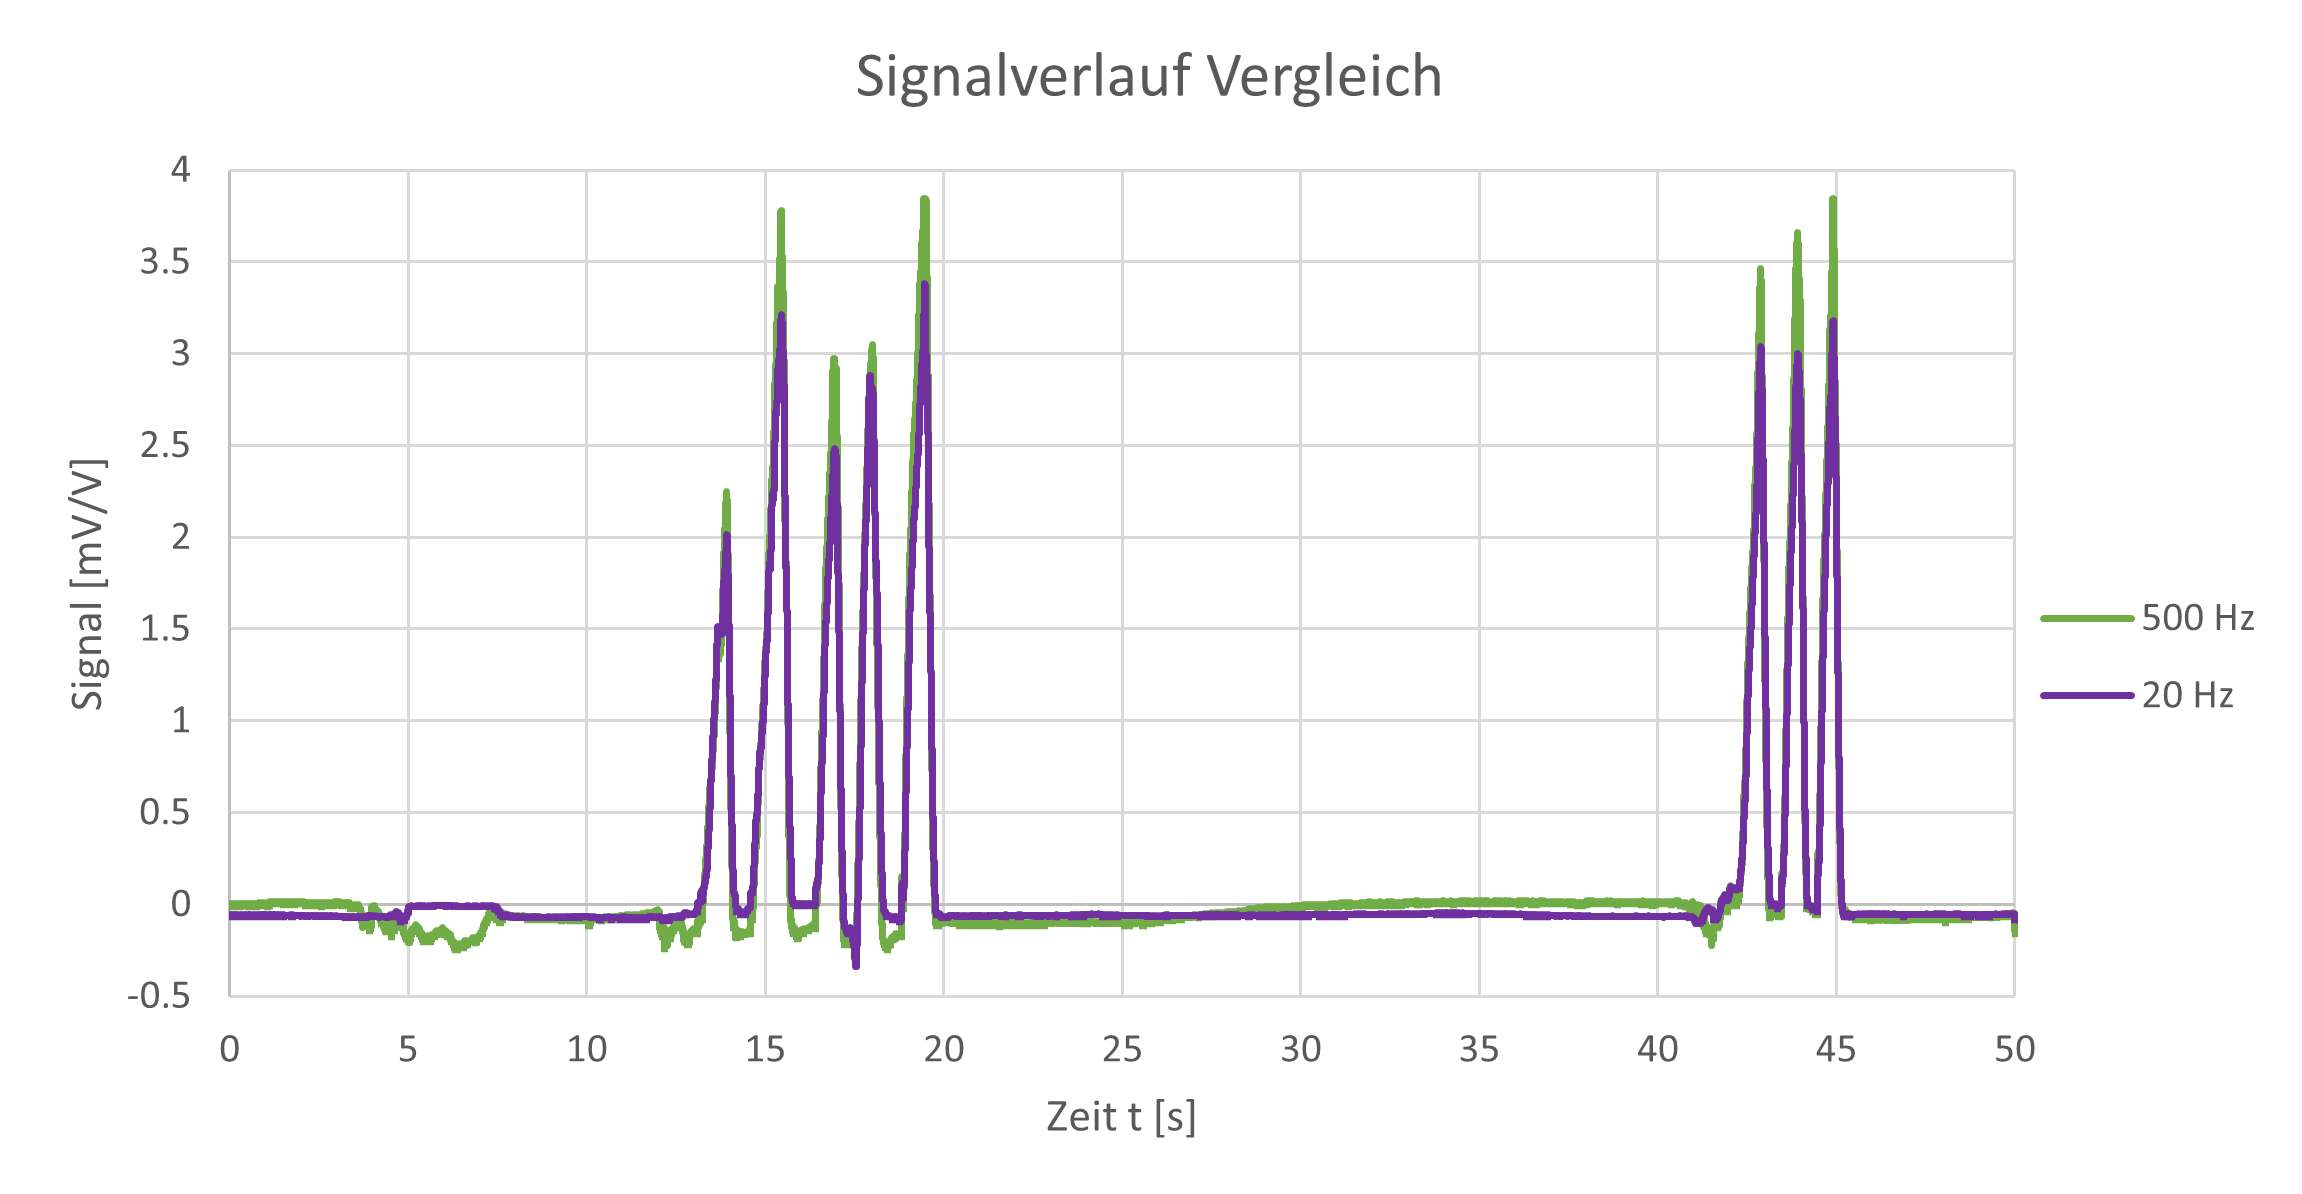
\includegraphics[width=1\linewidth]{imgs/daten_008_kpl}
	\caption{500 Hz (Unvergossen) vs 20 Hz (unvergossen) bei vergleichbarer Belastung}
	\label{fig:daten008kpl}
\end{figure}
	
\end{document}